

%----------------------------------------------------------------------------------------
%	PACKAGES AND OTHER DOCUMENT CONFIGURATIONS
%----------------------------------------------------------------------------------------

\documentclass{article}

\usepackage{fancyhdr} % Required for custom headers
\usepackage{lastpage} % Required to determine the last page for the footer
\usepackage{extramarks} % Required for headers and footers
\usepackage[usenames,dvipsnames]{color} % Required for custom colors
\usepackage{graphicx} % Required to insert images
\usepackage{listings} % Required for insertion of code
\usepackage{courier} % Required for the courier font
\usepackage[table]{xcolor}
\usepackage{multirow}
\usepackage{tabularx}
\usepackage{hyperref}

% Margins
\topmargin=-0.45in
\evensidemargin=0in
\oddsidemargin=0in
\textwidth=6.5in
\textheight=9.0in
\headsep=0.25in

\linespread{1.1} % Line spacing

% Set up the header and footer
\pagestyle{fancy}
\lhead{\hmwkAuthorName\ : \hmwkStudentID} % Top left header
\chead{ \hmwkClassShort} % Top center head
\rhead{\firstxmark } % Top right header
\lfoot{\lastxmark} % Bottom left footer
\cfoot{} % Bottom center footer
\rfoot{Page\ \thepage\ of\ \protect\pageref{LastPage}} % Bottom right footer
\renewcommand\headrulewidth{0.4pt} % Size of the header rule
\renewcommand\footrulewidth{0.4pt} % Size of the footer rule

\setlength\parindent{0pt} % Removes all indentation from paragraphs

%----------------------------------------------------------------------------------------
%	CODE INCLUSION CONFIGURATION
%----------------------------------------------------------------------------------------

\definecolor{MyDarkGreen}{rgb}{0.0,0.4,0.0} % This is the color used for comments
\lstloadlanguages{C} % Load Perl syntax for listings, for a list of other languages supported see: ftp://ftp.tex.ac.uk/tex-archive/macros/latex/contrib/listings/listings.pdf
\lstset{language=SQL, % Use c in this example
        frame=single, % Single frame around code
        basicstyle=\small\ttfamily, % Use small true type font
        keywordstyle=[1]\color{Blue}\bf, % cfunctions bold and blue
        keywordstyle=[2]\color{Purple}, % c function arguments purple
        keywordstyle=[3]\color{Blue}\underbar, % Custom functions underlined and blue
        identifierstyle=, % Nothing special about identifiers                                         
        commentstyle=\usefont{T1}{pcr}{m}{sl}\color{MyDarkGreen}\small, % Comments small dark green courier font
        stringstyle=\color{Purple}, % Strings are purple
        showstringspaces=false, % Don't put marks in string spaces
        tabsize=5, % 5 spaces per tab
        %
        % Put standard c functions not included in the default language here
        morekeywords={rand},
        %
        % Put c function parameters here
        morekeywords=[2]{on, off, interp},
        %
        % Put user defined functions here
        morekeywords=[3]{test},
       	%
        morecomment=[l][\color{Blue}]{...}, % Line continuation (...) like blue comment
        numbers=left, % Line numbers on left
        firstnumber=1, % Line numbers start with line 1
        numberstyle=\tiny\color{Blue}, % Line numbers are blue and small
        stepnumber=1 % Line numbers go in steps of 5
}

% Creates a new command to include a script, the first parameter is the filename of the script (without .txt), the second parameter is the caption
\newcommand{\Cscript}[2]{
\begin{itemize}
\item[]\lstinputlisting[caption=#2,label=#1]{#1.txt}
\end{itemize}
}
\renewcommand{\arraystretch}{1.5}

%----------------------------------------------------------------------------------------
%	DOCUMENT STRUCTURE COMMANDS
%	Skip this unless you know what you're doing
%----------------------------------------------------------------------------------------

% Header and footer for when a page split occurs within a problem environment
\newcommand{\enterProblemHeader}[1]{
\nobreak\extramarks{#1}{#1 continued on next page\ldots}\nobreak
\nobreak\extramarks{#1 }{#1 continued on next page\ldots}\nobreak
}

% Header and footer for when a page split occurs between problem environments
\newcommand{\exitProblemHeader}[1]{
\nobreak\extramarks{#1}{#1 continued on next page\ldots}\nobreak
\nobreak\extramarks{#1}{}\nobreak
}

\setcounter{secnumdepth}{0} % Removes default section numbers
\newcounter{homeworkProblemCounter} % Creates a counter to keep track of the number of problems

\newcommand{\homeworkProblemName}{}
\newenvironment{homeworkProblem}[1][Problem \arabic{homeworkProblemCounter}]{ % Makes a new environment called homeworkProblem which takes 1 argument (custom name) but the default is "Problem #"
\stepcounter{homeworkProblemCounter} % Increase counter for number of problems
\renewcommand{\homeworkProblemName}{#1} % Assign \homeworkProblemName the name of the problem
\section{\homeworkProblemName} % Make a section in the document with the custom problem count
\enterProblemHeader{\homeworkProblemName} % Header and footer within the environment
}{
\exitProblemHeader{\homeworkProblemName} % Header and footer after the environment
}

\newcommand{\problemAnswer}[1]{ % Defines the problem answer command with the content as the only argument
\noindent\framebox[\columnwidth][c]{\begin{minipage}{0.98\columnwidth}#1\end{minipage}} % Makes the box around the problem answer and puts the content inside
}

\newcommand{\homeworkSectionName}{}
\newenvironment{homeworkSection}[1]{ % New environment for sections within homework problems, takes 1 argument - the name of the section
\renewcommand{\homeworkSectionName}{#1} % Assign \homeworkSectionName to the name of the section from the environment argument
\subsection{\homeworkSectionName} % Make a subsection with the custom name of the subsection
\enterProblemHeader{\homeworkProblemName} % Header and footer within the environment
}{
\enterProblemHeader{\homeworkProblemName} % Header and footer after the environment
}

%----------------------------------------------------------------------------------------
%	NAME AND CLASS SECTION
%----------------------------------------------------------------------------------------

\newcommand{\hmwkTitle}{220CT Data and Information Retrieval\\ Coursework} % Assignment title
\newcommand{\hmwkDueDate}{March 13th 2015} % Due date
\newcommand{\hmwkClass}{ECU178 \- Computer Science} % Course/class
\newcommand{\hmwkClassTime}{10:30am} % Class/lecture time
\newcommand{\hmwkClassInstructor}{} % Teacher/lecturer
\newcommand{\hmwkAuthorName}{Robert Rigler} % Your name
\newcommand{\hmwkStudentID}{4939377}% My Student ID
\newcommand{\hmwkClassShort}{220CT Coursework } %Short name for class (only used in header)

%----------------------------------------------------------------------------------------
%	TITLE PAGE
%----------------------------------------------------------------------------------------

\title{
\vspace{2in}
\textmd{\textbf{\hmwkClass:\ \\ \hmwkTitle}}\\
\normalsize\vspace{0.1in}\small{Due\ on\ \hmwkDueDate}\\
\vspace{0.1in}\large{\textit{\hmwkClassInstructor\ }}
\vspace{3in}
}

\author{\textbf{\hmwkAuthorName\ : \hmwkStudentID}}
\date{} % Insert date here if you want it to appear below your name

%----------------------------------------------------------------------------------------

\begin{document}

\maketitle

%----------------------------------------------------------------------------------------
%	TABLE OF CONTENTS
%----------------------------------------------------------------------------------------

%\setcounter{tocdepth}{1} % Uncomment this line if you don't want subsections listed in the ToC

\newpage
\tableofcontents
\newpage

%----------------------------------------------------------------------------------------
%	Problem 1
%----------------------------------------------------------------------------------------
\begin{homeworkProblem}[Task 1 Database Design]
	This task in Database Design consists of four activities. The first three involve normalising the given data to third normal form, and the fourth is to produce and Entity Relationship diagram of the normalised relations.\\
		For each activity I will give a detailed step by step explanation of how I completed each activity. 
		
		
	\begin{homeworkSection}{Activity 1: First Normal Form}{
		
		To put this data into First Normal Form (1NF), I need to:
		\begin{enumerate}
			\item Identify any repeating redundant data and remove it from the current Entity
			\item Place the data into a new Entity
			\item Create a relationship with a primary key from one Entity as a foreign key in the other.
		\end{enumerate}
			
			\subsubsection{Step 1: Identify Redundancy}
				
		On inspecting the data, I can see that there are multiple instances of repeating data.\\ Orders' ID: \emph{CON-2237, CON-2356} and \emph{CON-1234}  all  have repeating data entries for fields:
		 \emph{Equipment, Qty,} and \emph{Unit Price} .
		 
		 \subsubsection{Step 2: Create New Entity}
		 
		 Removing the \emph{Equipment, Qty,} and \emph{Unit Price} fields and placing them in a new entity, leaves me with two entities as shown below.\\
		 
		
		 
		
		 
		 
		
		 
		\subsubsection{Step 3: Relationships and Keys}
		
		To complete the First Normal Form, a relationship needs to be created between the entities.
		
		 I created the relationship by including the \textit{Order ID} attribute as a foreign key in the \textit{ItemOrder} entity.\\
		\textit{Order ID} is used as a Primary Key for the \textit{Order} entity.
		In the \emph{ItemOrder} entity, no one attribute can be used to uniquely identify a single record. For this reason, I have created a concatenated key using the attributes \emph{Equipment} and \emph{Order ID}. The concatenated key can now be used to uniquely identify each record.\\
		
		\subsubsection{1NF : Diagram}
		 \begin{tabular}{l r| c c c c l r|} Order & $($ \underline{Order ID} & & & & & ItemOrder & $($ \underline{*Order ID}\\
		 	& Supplier ID	& & & & & & \underline{Equipment} \\
		 	& Client Name & & & & & & Qty $)$\\
		 	& Client Address  & & & & & & Unit Price $)$\\
		 	& Date\\
		 	& Total Price$)$\\
		 \end{tabular}
		 
		\pagebreak
		
		 \subsubsection{1NF :  Data}
		 \hspace{7.5cm}\textit{Order} entity
		 
		  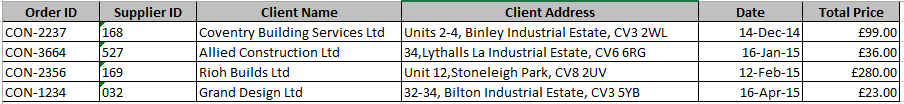
\includegraphics[ width=1\columnwidth, height=3cm]{Task1/Order1NF.png}
		  
		  \vspace{10px}
		  
		 \hspace{4cm} \emph{ItemOrder} entity\\
		 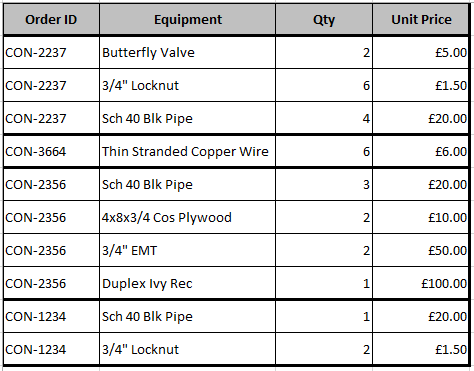
\includegraphics[scale = 0.8]{Task1/Item11NF.png}
			}
		
		
	
	\end{homeworkSection}
	
	\pagebreak
	
	\begin{homeworkSection}{Activity 2: Second Normal Form}
		To put this data into the Second Normal Form(2NF) I need to ensure that the attributes are completely dependant on the primary key, i.e., that no attribute is only dependant on one part of the primary key.\\
		This can be done in two steps:
		\begin{enumerate}
			\item Test each attribute for complete dependency on the primary key.
			\item Remove any partially dependent attributes to a new entity and assign a primary key.
		\end{enumerate}
		
		For this particular set of data, the \emph{Order} entity does not have a concatenated key and therefore is already in the second normal form.
		
		\subsubsection{Step 1: Testing each attribute.} \vspace{10px}
		
		\begin{center}
			
			
			
			\begin{tabular}{|l|c|l|}
				\hline
				\textbf{	Primary Key} & \textbf{Attribute} & \textbf{Functionally Dependant?}\\ \hline
				Order ID, Equipment & Qty & Yes, dependant on both\\ \hline
				Order ID, Equipment & Unit Price & No, dependant on Equipment only\\ \hline
			\end{tabular}
			
		\end{center}
		\subsubsection{Step 2: Entity, Relationship and Key }
		
		From my testing, I found that the attribute \emph{Unit Price} is not functionally dependant as it is only dependent on \textit{Equipment}, but not\textit{ Order ID}.\\
		 I moved \emph{Equipment} and \textit{Unit Price} into a new entity called \textit{Item} and made \textit{Equipment} the primary key. \\ I created a relationship between the \textit{Item} and \textit{ItemOrder} entities by repeating the \textit{Equipment} attribute in \textit{ItemOrder} as a foreign key.
		
		\vspace{10px}
		
		
		
		\subsubsection{Entities in Second Normal Form: Diagram}
		
		\begin{tabular}{l r |c c c c l r| c c c l r|}
		
		{\textbf{Order}} &$($ \underline{Order ID} & & & & & \textbf{Item} & $($ \underline{Equipment} & & & & \textbf{ItemOrder}& $($\underline{*Order ID}  \\
			& Suppler ID & & & & & & Unit Price$)$ & & & & & \underline{*Equipment}\\
			& Client Name & & & & & & & & & & & Qty $)$\\
			& Client Address & & & & & \\
			& Date & & & & & \\
			& Total Price $)$ & & & & & \\
			  
		\end{tabular}
		\pagebreak
		\subsubsection{Entities in Second Normal Form: With data}
	\centering \textit{Order} entity
		
		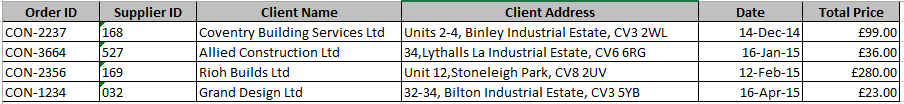
\includegraphics[ width=1\columnwidth, height=3cm]{Task1/Order1NF.png}
		\vspace{20px}
		\begin{center}
				\textit{Item} entity
				
				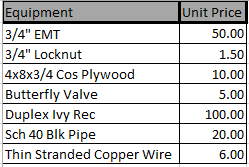
\includegraphics[scale = 1]{Task1/Item02.png}
	
		
		\vspace{20px}
		\textit{ItemOrder} entity
		
		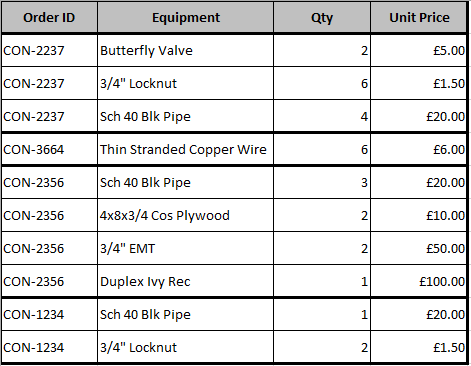
\includegraphics[scale = 0.7]{Task1/Item12NF.png}
		\end{center}
		
		\pagebreak
	\end{homeworkSection}
	\begin{homeworkSection}{Activity 3: Third Normal Form}
		
		To place the data into Third Normal Form 3NF I need to ensure that all attributes are only dependent on the Primary Key, and not Non-Key Attributes.
		This can be achieved in two steps:
		
		\begin{enumerate}
			\item Test each attribute for dependency on the primary key.
			\item Remove all transitive dependencies to a new entity with the correct primary key and relationship.
		\end{enumerate}
		
		For this particular set of data, both the \emph{Item} and \textit{ItemOrder} entities are already in the Third Normal Form.
		
		\subsubsection{Step 1: Testing for Transitive Dependency}
		
		\emph{Order} Entity
		
		\begin{tabular}{|l|l|l|}
			\hline
			\textbf{Primary Key} & \textbf{Attribute} & \textbf{Transitive Dependency?}  \\\hline
			Order ID & Supplier ID & Yes: Supplier ID can be found if we know Client Name or Address \\\hline
			Order ID & Client Name & Yes: Client Name can be found if we know Supplier ID or Address  \\\hline
			Order ID & Client Address & Yes: Client Address can be found if we know Client Name or Supplier ID   \\\hline
			Order ID & Date & No: Only dependent on Primary Key  \\\hline
			Order ID & Total Cost& No: Only dependent on Primary Key \\\hline
		\end{tabular}
		\vspace{10px}
		
		Using this table I have identified that \textit{Supplier ID, Client Name,} and\textit{ Client Address} all have transitive dependencies, and need to be moved to a new entity.
		
		\subsubsection{Step 2: Entity, Relationship and Key}
		
		I created a new entity called \textit{Customer}, and moved the three attributes with transitive dependencies into it. I then made \textit{Supplier ID} the Primary Key and created a relationship between the \textit{Customer} and \textit{Order} entities by repeating the \textit{Supplier ID} attribute as a foreign key in the \textit{Order} entity.\\
	
			\subsubsection{Entities in Third Normal Form: Diagram}
			
		\begin{tabular}{l r |c c c c l r| c c c l r|}
			
			{\textbf{Order}} &$($ \underline{Order ID} & & & & & \textbf{Item} & $($ \underline{Equipment} & & & & \textbf{ItemOrder}& $($\underline{*Order ID}  \\
			& *Suppler ID & & & & & & Unit Price$)$ & & & & & \underline{*Equipment}\\
			& Date& & & & & & & & & & & Qty $)$\\
			& Total Price $)$  
			
		\end{tabular}
		
		
				\vspace{40px}
				
		\begin{tabular}{l r|}
			\textbf{Customer} & $($ \underline{Supplier ID} \\
			& Client Name\\
			& Client Address $)$\\
		\end{tabular}		
		\pagebreak
		\subsubsection{Entities in Third Normal Form: With Data}
		\begin{center}
			
			\textit{Order} entity
			
			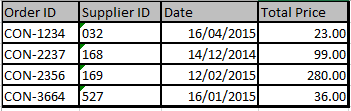
\includegraphics[scale = 0.8]{Task1/03.png}
			
			\vspace{10px}
			\textit{Item} entity
			
			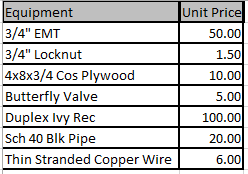
\includegraphics[scale = 0.8]{Task1/I3.png}
			
			\vspace{20px}
			\textit{ItemOrder} entity
			
			
			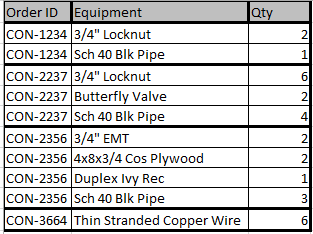
\includegraphics[scale = 0.8]{Task1/IO3.png}
			
			\vspace{20px}
			\textit{Customer} entity
			
			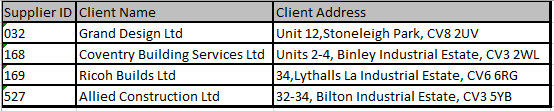
\includegraphics[scale = 0.8]{Task1/C3.png}
		\end{center}
		\pagebreak
		
		
	\end{homeworkSection}
	\begin{homeworkSection}{Activity 4: ER Diagram}
		
		
	\end{homeworkSection}
	\end{homeworkProblem}

\begin{homeworkProblem}[Task 2: Database Development]
	For this task I will provide the SQL statement I used to complete each question activity, I will then explain each part of the SQL statement, and give screen-shots of before and after the statement was executed (if applicable).\\
	Each SQL statement was written and tested using ORACLE 11g Express Edition and ORACLE Application Express.
	\begin{homeworkSection}{Question 1 }
		
		To begin I created the two tables which have no dependency on any other table: \textit{Aircraft} and \textit{Airline}\\
		
		\subsubsection{Aircraft}
	\Cscript{Task2/C_a}{CREATE AIRCRAFT}
	
	The statement begins with \textit{'CREATE TABLE Aircraft'} which will create a table called \textit{aircraft}. Inside the brackets the three fields, their data types, and any constraints are listed. Below is a table which will explain why I chose these data types and constraints for each field.   
	
	\vspace{1.5cm}
	\begin{tabular}{|l|c|l|p{8cm}|}\hline \textbf{Identifier} & \textbf{Data-Type} &\textbf{Constraint} & \textbf{Explanation} \\ \hline 
		aircraft\textunderscore code & VARCHAR2(5) & PRIMARY KEY & All aircraft\textunderscore codes start with 'C' and are followed by up to four numerical digits. This field will be used as the Primary Key of the table.\\ 
		aircraft\textunderscore type & VARCHAR(30) & NOT NULL & Contains a combination of alphanumeric characters of up to 30 characters in length. This field cannot be left empty.\\
		aircraft\textunderscore price & NUMBER(11,2) & NOT NULL & Stores large numeric values, with a  precision of 11 and a scale of 2. This allows for prices up to 99 Thousand Million and two decimal places. This field cannot be left empty.\\\hline
		
	\end{tabular}
	\pagebreak
	
	
	\subsubsection{Airline}
	\Cscript{Task2/C_ac}{CREATE AIRLINE}
	
	\begin{tabular}{|l|l|l|p{8cm}|}\hline \textbf{Identifier} & \textbf{Data-Type} &\textbf{Constraint} & \textbf{Explanation} \\ \hline 
	airline\textunderscore code & CHAR(4) & PRIMARY KEY & A combination of 4 alphanumeric characters.    airline\textunderscore code is also the Primary Key\\
	airline\textunderscore name & VARCHAR2(20) & NOT NULL &  This field allows a variable length of characters, up to a maximum of 20. This field cannot be left empty. \\
	airline\textunderscore address & VARCHAR2(60) & NOT NULL & This field allows for a combination of alphanumeric characters up to a maximum length of 60. This field cannot be left empty.\\
	airline\textunderscore city & VARCHAR2(15) & NOT NULL & This field allows a combination of alphanumeric characters up to a maximum length of 15. This field cannot be left empty.\\
	airline\textunderscore country & VARCHAR2(15) & NOT NULL & This field allows for a combination of alphanumeric characters up to a maximum length of 15. This field cannot be left empty.\\
		\hline
	\end{tabular}
	
	\pagebreak
	
	\subsubsection{Purchase\textunderscore Order}
	

	\Cscript{Task2/c_P}{CREATE PURCHASE\textunderscore ORDER}
	
\begin{tabularx}{\textwidth}{|l|l|p{3cm}|X|}\hline \textbf{Identifier} & \textbf{Data-Type} &\textbf{Constraint} & \textbf{Explanation} \\ \hline 
	purchase\textunderscore order\textunderscore no & NUMBER(3,0) & PRIMARY KEY & This field allows for numeric input with a precision of 3 and a scale of 0, this allows values in the range of 001 to 999. This field also acts as the Primary Key.\\
	airline\textunderscore code & CHAR(4) & NOT NULL,\newline FOREIGN KEY & A combination of 4 alphanumeric characters. This field is a foreign key; Referencing the \textit{airline\textunderscore code} field from the \textit{Airline} table.\\
	date\textunderscore of\textunderscore purchase & DATE & NOT NULL\\
	\hline
\end{tabularx}
	
	
	\pagebreak
	\subsubsection{Ordered\textunderscore Aircraft}
	
	\Cscript{Task2/C_Oa}{CREATE ORDERED\textunderscore AIRCRAFT}
	
	\begin{tabularx}{\textwidth}{|l|l|p{2.7cm}|X|}\hline \textbf{Identifier} & \textbf{Data-Type} &\textbf{Constraint} & \textbf{Explanation} \\ \hline 
		
	purchase\textunderscore order\textunderscore no & NUMBER(3,0) & NOT NULL, PRIMARY KEY, FOREIGN KEY & This field allows for numeric input with a precision of 3 and a scale of 0. It is a foreign key referencing; $purchase\textunderscore order\textunderscore no$ from $purchase\textunderscore order$\\
	
	aircraft\textunderscore code & VARCHAR2(5) & NOT NULL, PRIMARY KEY, FOREIGN KEY& This field allows for alphanumeric input up to a maximum length of 5. It is part of a composite key and is also a foreign key referencing $aircraft\textunderscore code$ from $aircraft$.  \\
	aircraft\textunderscore quantity. & NUMBER (3,0) & NOT NULL & This field allows for 3 digit numbers. This field cannot be left blank.\\
	
		\hline
	\end{tabularx}
	
	\end{homeworkSection}
	\pagebreak
	\begin{homeworkSection}{Question 2}
		


		\subsubsection{Aircraft}
		
		\Cscript{Task2/I_aircraft}{INSERT INTO \textit{AIRCRAFT}}
		
		The SQL statement uses the following pattern:\\ \textit{INSERT ALL...INTO (\textit{table identifier}) VALUES (\textit{data})} .\\ \\This allows me to input multiple records into the table simultaneously. '\textit{INTO Aircraft}' specifies that I am going to insert the following values into the \textit{Aircraft} table. \\The text in brackets following the word \textit{VALUES} is the data which is input into that record.\\\\
		\textit{'SELECT 1 FROM DUAL'} is a requirement of INSERT ALL, so that it can function correctly.
		\vspace{1cm}
		
		 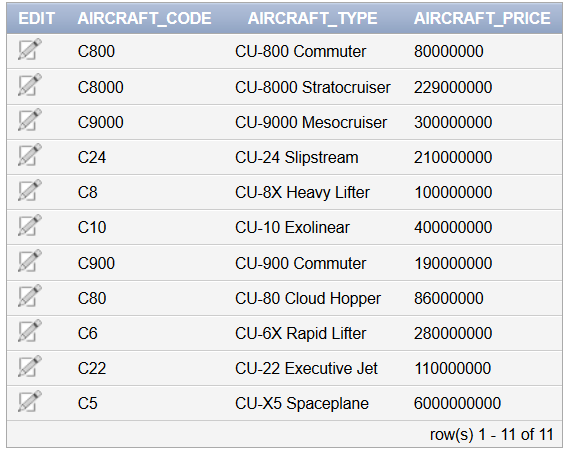
\includegraphics[scale = 0.55]{Task2/I_aircraft.png}
		
		
		\pagebreak
		\subsubsection{Airline}
	 
		\Cscript{Task2/I_airline}{INSERT INTO \textit{AIRLINE}}
		
		\vspace{1cm}
		
		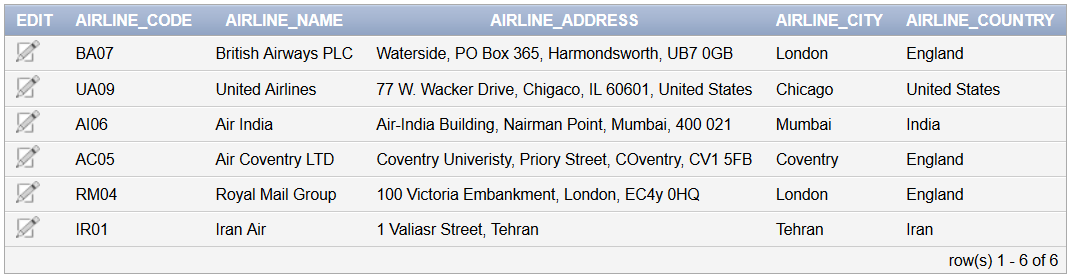
\includegraphics[scale = 0.5]{Task2/I_airline.png}
		
		\pagebreak
		\subsubsection{Purchase\textunderscore Order}
		
		\Cscript{Task2/I_purchase_order}{INSERT INTO \textit{PURCHASE\textunderscore ORDER}}
		
		\vspace{1cm}
		
		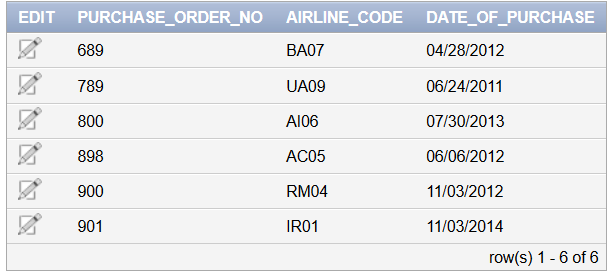
\includegraphics[scale = 0.55]{Task2/I_purchaseorder.png}
		
		
		\pagebreak
		
		\subsubsection{Ordered\textunderscore Aircraft}
			
		\Cscript{Task2/I_ordered_aircraft}{INSERT INTO \textit{ORDERED\textunderscore AIRCRAFT}}
		
		
		
		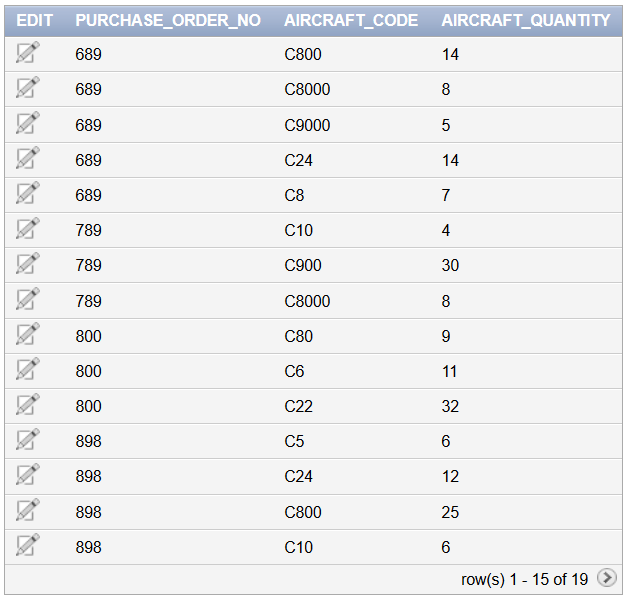
\includegraphics[scale = 0.5]{Task2/I_orderedaircraft.png}
		
		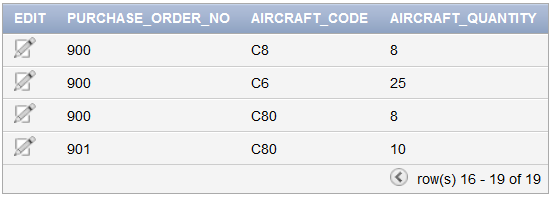
\includegraphics[scale = 0.55]{Task2/q21.png}
		\pagebreak
	\end{homeworkSection}
	
	\begin{homeworkSection}{Question 3}
		
		This question requires me to find the; Average, Minimum and Maximum price for all aircraft bought after '01/01/2012'.
		
		
		\Cscript{Task2/Q3}{AVG() MIN() MAX()}
		
		Firstly, to work out the price for all the aircraft bought, I multiply the quantity of aircraft ordered\\ (\textit{aircraft\textunderscore quantity}) by the price of that particular aircraft (\textit{aircraft\textunderscore price}). To find the average, minimum and maximum of these prices then I need to use this calculation in conjunction with the \textcolor{blue}{\textit{AVG()}}, \textcolor{blue}{\textit{MIN()}} and \textcolor{blue}{\textit{MAX()}} SQL functions respectively. These functions will perform this calculation on every record in the specified tables and return the correct value. Once I selected the values, I used the \textcolor{blue}{\textit{AS}} keyword to label the output columns. \\ This can be seen in line 1 - 3 in the code above.
		\\
		In total, this SQL statement uses three tables	\textit{ordered\textunderscore aircraft} and \textit{aircraft} for the calculations, and \textit{purchase\textunderscore order} for the conditional statement.\\
		To be able to use the data from multiple tables, I need to use \textcolor{blue}{\textit{JOINS}}. \textcolor{blue}{\textit{JOINS}} allow me to combine common records from two or more tables by using the syntax structure;\\\\ \textcolor{blue}{\textit{JOIN}} \textit{table name} \textcolor{blue}{\textit{ON}} \textit{table1.attribute = table2.attribute}\\\\
		For this problem I used two joins;
		\begin{enumerate}
			\item  \textcolor{blue}{JOIN} aircraft
			\textcolor{blue}{ON} ordered\textunderscore aircraft.aircraft\textunderscore code = aircraft.aircraft\textunderscore code
			\item \textcolor{blue}{JOIN} purchase\textunderscore order
			\textcolor{blue}{ON} ordered\textunderscore aircraft.purchase\textunderscore order\textunderscore no = purchase\textunderscore order.purchase\textunderscore order\textunderscore no
		\end{enumerate}
		
		
		
		Join number One is used to select the correct relation attributes from both required tables.\\
		Join number Two is used to ensure that the \textcolor{blue}{WHERE} condition relates to the selected attributes.
		
		This allowed me to select all the values I needed and also make sure that the value used in each calculation were from the same record. 
		
	
		Below is a screenshot of the statements' output.\vspace{1cm}
		
		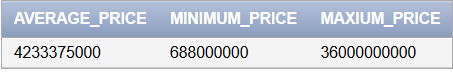
\includegraphics[scale = 0.8]{Task2/Q3.png} 
		
		
		\pagebreak
		
		\begin{homeworkSection}{Question 4}
			This question required me to: "Display the purchase order number, date, airline name, address, airline country for airlines where the total cost of an order is less than 10,000 million pounds.  Your results should be in descending alphabetical order based on the airline code".\\
			
			\Cscript{Task2/Q4}{Question 4}
			
			
			Lines 1 - 8 above I am using a \textcolor{blue}{SELECT} ... \textcolor{blue}{FROM} statement to select the required atributes from the tables. However not all of these attributes are from the same table, so I used multiple \textcolor{blue}{JOIN} statements (lines 9 - 14) to combine the common attributes. On line 15 I used a \textcolor{blue}{WHERE} keyword to specify the required condition (Total cost > 10,000 Million pounds). Finally on Line 16, I sorted the results in descending order on \textit{airine\textunderscore code} by using \textcolor{blue}{ORDER BY} \textcolor{blue}...{DESC}.
			\\
			Below is a screenshot of the statements' output.
			
			\vspace{1cm}
			
			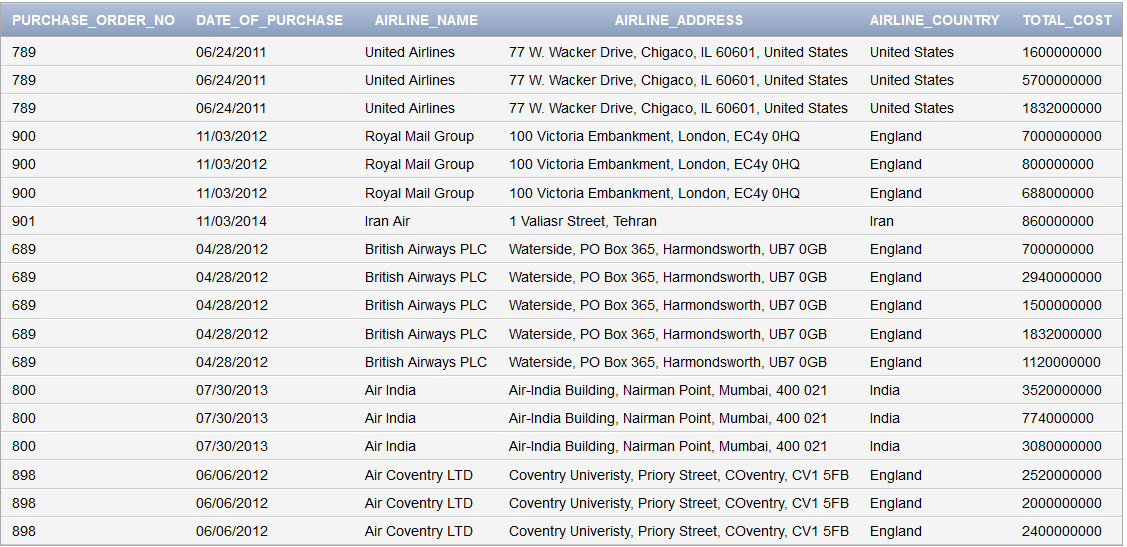
\includegraphics[scale = 0.4]{Task2/q4.png} 
			\pagebreak
			
		\end{homeworkSection}
		
		\begin{homeworkSection}{Question 5}
			This question required me to: "Display how many aircraft were ordered by British Airways in total and by each different airplane type."\\
			
			\Cscript{Task2/Q5}{Question5}
			
			Lines 1 - 3 use \textcolor{blue}{SELECT} ... \textcolor{blue}{FROM} to select the two rows needed for this task.\\
			Lines 4 - 9 contains the joins required to combine the related data in the tables.\\
			Lines 10 uses \textcolor{blue}{WHERE} to define a condition. In this particular case it only selects data where airline\textunderscore code is equal to $BA07$ , which is the airline code for \textit{"British airways PLC"}.\\
			Below is a screenshot of the statements' output.
			\vspace{1cm}
			
			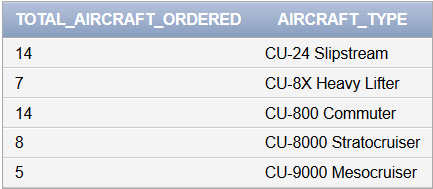
\includegraphics{Task2/q5}
			\pagebreak
		\end{homeworkSection}
		
		\begin{homeworkSection}{Question 6}
			
			This question required me to: "Produce a list of all the orders from all the airlines. The list should show the airline code, followed by the order number, followed by the code of the aircraft ordered, followed by the quantity of aircraft ordered and then the total cost of that order. The list should be arranged by airline code in descending order."
			
			\Cscript{Task2/Q6}{Question 6}
			
			Lines 1 - 7 use \textcolor{blue}{SELECT} ... \textcolor{blue}{FROM} to select the five rows needed for this task and specify their location.\\
			Lines 8 - 13 join the tables so to combined the related data to achieve contiguous output.\\
			Line 14 \textcolor{blue}{ORDER BY} \textcolor{blue}...{DESC} to sort the data in descending order via the \textit{airline\textunderscore code} column.\\
			Below is a screenshot of the statements' output.
			\vspace{1cm}
			
			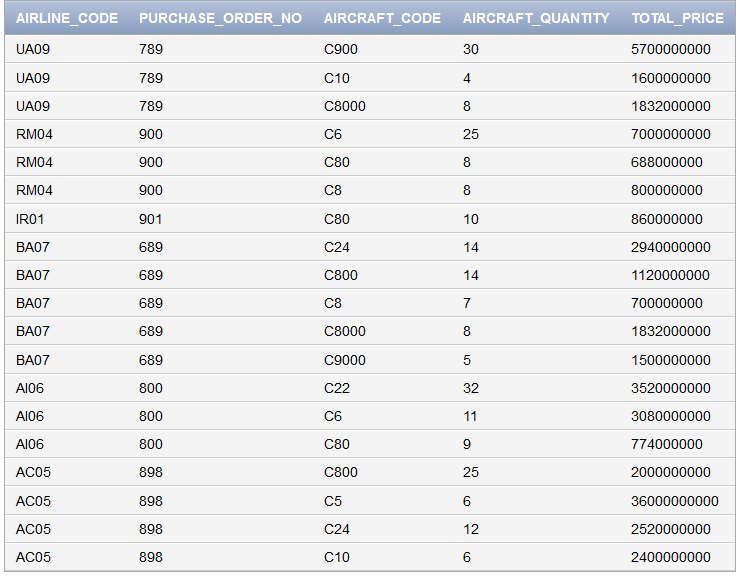
\includegraphics[scale =0.5]{Task2/q6}
			\pagebreak
		\end{homeworkSection}
		
		
	\end{homeworkSection}
	
	\begin{homeworkSection}{Question 7}
		This question required me to : ". Display the order details, airline details and the aircraft details where more than 10 aircraft of a specific type were ordered."\\
		
		\Cscript{Task2/Q7}{Question 7}
		
		Lines 1 - 10 select the required rows from the data tables.\\
		Lines 11 - 16 Joins the tables on the common data elements.
		\\Line 17 is a condition statement, where the \textit{aircraft\textunderscore quantity} is greater than ten.\\
		Below is a screenshot of the statements' output.
		\vspace{1cm}
		
		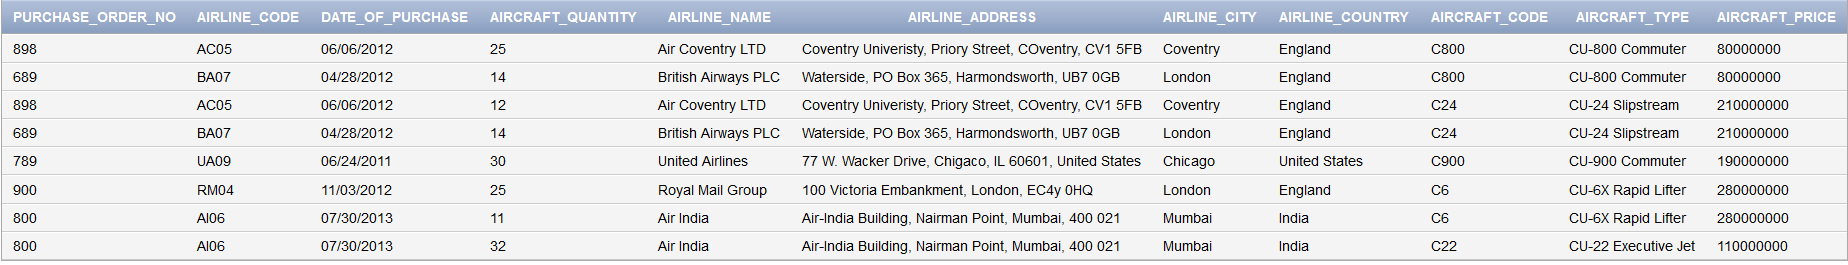
\includegraphics[width=\columnwidth, height = 4cm]{Task2/q7}
		\pagebreak
	\end{homeworkSection}
	
	\begin{homeworkSection}{Question 8}
		
		This question required me to: "We have discovered an error in our spreadsheet. The C800 aircraft should have been 100 million not 80 million please update the database based on this change."
		
		\Cscript{Task2/Q8}{Question 8}
		
		Below is a screen shot of the updated record.
		\vspace{1cm}
		
		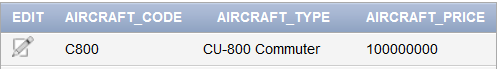
\includegraphics[scale = 0.7]{Task2/Q8}
		
	\end{homeworkSection}
	
	\begin{homeworkSection}{Question 9}
		
		
			This question required me to: ". Air Coventry LTD has changed its name to Coventry University Airways please update the information."
			
			\Cscript{Task2/Q9}{Question 9}
			
			Below is a screen shot of the updated record.
			\vspace{1cm}
			
			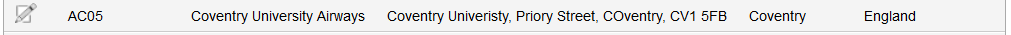
\includegraphics[scale = 0.5]{Task2/q9}
			
		\end{homeworkSection}
	
	
\end{homeworkProblem}


\pagebreak
\begin{homeworkProblem}[Task 3 : Poster of Ethics]

\end{homeworkProblem}

\pagebreak

\begin{homeworkProblem}[Task 4 : Amazon recommendation system]
	
	\begin{homeworkSection}{What is a Recommendation System?}
		
		Recommendation systems are commonly described as:\\\\  "\textit{A way of presenting information on items and products that are likely to be of interest to the reader.}" $[1]$\\
		 
		 
		 
		 Recommendation systems work via the use of Data Mining. Data Mining is  a process where data is gathered and analysed to find specific patterns. These patterns can provide meaningful and insightful data which can then be relayed to the consumer.\\
		 
		 The data gathered for a recommendation system comes in many varieties and is often tailored to the recommendation systems' main purpose. For Example, a system may collect data on a users' Hobbies, Interests, Opinions, Habits, Recent search history, Recent Purchase History and many more areas.
		 \\
		 
	
	\end{homeworkSection}
	
	\begin{homeworkSection}{Data Gathering and Preparation}
	Amazon is an incredibly popular E-Commerce website which caters to millions of customers everyday. This is partially due to its intricate and extensive data mining operations which result in a very effective recommendation system. The effectiveness of this system can be seen by looking at their percentage sales increases;\\\\ "The company reported a 29\% sales increase to \$12.83 billion during its second fiscal quarter, up from \$9.9 billion during the same time last year."$[2]$\\
	
	
		\subsubsection{Data}
		To make the recommendation system as effective as possible, Amazon must collect a huge amount of data on each customer and more importantly they must collect the right data. In this section I will explore what kind of data this recommendation system should collect.\\
		At Amazon, the recommendation system is used to personalize the shopping environment for each customer, so the store changes drastically depending on the customer.
		
		\begin{description}
			\item[Completed Purchases] \hfill\\
				Products the customer has spent money on.
			\item [Incomplete purchases]\hfill \\
				Abandoned shopping carts or specific items dropped from the cart.
			\item [Personal item ratings/reviews]\hfill \\
				Ratings will change the recommendations depending on the quality of the rating.
			\item [Demographic information]\hfill \\
			Such as Location, Age, Profession, Type of education etc... will offer different recommendations depending on which demographic criteria the customer meets.
			\item [Number of views]\hfill \\
			How many times was that particular item, or similar items viewed before purchase.
			\pagebreak
			\item [Time spent before purchase]\hfill \\
			How long it takes for a customer to purchase an item
			\item [Click-Through Rate]\hfill \\
			How often a customer clicks on a recommendation.
			\item [Conversion rate]\hfill \\
			How often the customer purchases an item that has been recommended.
			\item [Referrals]\hfill \\
			Did the customer arrive here from a different website, if so, that website could infer interest in specific items.
		\end{description}
		
		All of these possible information sources can be categorized into three main categories:
		\begin{description}
			\item[Demographic Data]\hfill \\ This is data about the customer, which can be used to identify them. e.g Age, Gender,Social class and Location.
			\item[Item Data]\hfill \\ This is data that can identify specific items or groups of related items. This may include keywords, tags, Genres and types.
			\item[User-Item Data] \hfill \\ This is explicit data, which is provided by the customer in the form of ratings and reviews. Ratings and reviews act as a linear scale on which a recommender system can use to recommend other items.
			
			
		\end{description}
		All of these types of data are in a web-format, meaning that all of the data here is collected via the consumers actions on the web page. The types of data that can be gather to include other external sources and formats. For example the recommendation system could be expanded to scrape information from the customers various social media profiles to gather more information.
		
	\end{homeworkSection}
	\pagebreak
	\begin{homeworkSection}{Benefits and limitations of a Recommendation system}
	
			Good recommendation systems drastically improve e-commerce sales, but there are also some downfalls. In this section I will explore both the benefits and limitations in detail. \hfill \\
			
			\subsection{Limitations}
			
			\begin{description}
				\item \textbf{Complexity}\hfill \\
				Making a system that produces relevant recommendations requires a lot of work. Primarily because there are so many variables that go into producing the most basic of recommendations. \hfill \\ It takes incredibly complex algorithms and a large amount of processing power to produce any recommendations at all. If the recommendation algorithm isn't at complex as it needs to be, or it doesn't use the right comparisons then it will only produce recommendations that are either very obvious or not of any interest at all. \hfill \\
				
				\item[Amount of Data]
				
				For recommendation systems to operate at their most effective, they need a large amount of accurate data. Not only do they need customer data, but also item data . Before a recommendation system is implemented a large amount of user data needs to be collected. This can prove difficult because sometimes that user data just isn't available. The more data a company can collect about their customers and about their own recommendation system results, the more accurate it will be. 
				
				\item[Data Accuracy]
				
					Data, by its nature is a rapidly expanding resource. Whilst the collection of data is a relatively simple process, deciding whether or not the data is relevant is far more complex. Hopefully, depending on the way the data is gathered, all of it will be relevant, but this is not always the case and valuable time and resources are used collecting and analysing this useless data.\\
					Not only may some of the data be irrelevant, some of it may be contradictory. For example if a customer changes some of his/her preferences or changes demographic, also shopping trends are always in flux i.e what was popular last week might not be the case a month from now. This inaccurate data will make the recommendation system less effective.
				
			\end{description}
			
			
			
			\subsection{Benefits}
			\begin{description}
				\item[Sales]\hfill \\
					An accurate recommendation system has the potential to increase sales and profits. This is done by giving the customer recommendations that they are interested in but did not plan to purchase, this increases average order value. \\ Once a customer has received personalized recommendations, overall customer retention (customer loyalty) increases.
					
				\item[Trends and Market data] \hfill \\
				The recommendation system doesn't just need a lot of data, it can also produce valuable data about shopping habits and market trends.
				This data can help drive the direction of the business to improve future sales and sales forecasting.
				\pagebreak
				\item[Real-Time Data]\hfill \\
				
				Similar to the section above, having data coming into the system in real time has many advantages. The data being collected is coming into the system in real time, this means that very little 'Guess-Work' needs to be done with predictions. The influx of new data means that recommendations can be updated almost instantaneously as soon as that data is available. Using current data minimises the potential for inaccurate or irrelevant predictions.
				
				\item[Automation]\hfill \\
				The recommendation system holds data about every  customer, it is continuously analysing their actions. Because of this, the users are effectively organizing their own content of the web page and deciding what they see in the future. The customer may not be away of this at all times, but this is very beneficial for the company. With the only participants being the system and the customers, a vast amount of the organisation and customer maintenance on the business side is reduced .
			\end{description}
	\end{homeworkSection}\pagebreak
	\begin{homeworkSection}{Analysis techniques}
		In this section I will explore how the types of data gathered above can be analysed to produce meaningful recommendations via \textit{ Association analysis}.\\
		
		Association analysis defines a broad spectrum of analytical techniques that focus on using complex algorithms to analyse large data sets to produce statistical rules that can explain the patterns within the data.\\
		
		\subsection{Collaborative filtering}
		
		Collaborative filtering is done by collecting specific data about the items that a customer has bought, and then comparing this data to that of other users. The recommendations produced are items that are liked by a user with similar purchase/rating data.\\
		
		The data needed for this approach is the explicit \textit{User-Item} data, which consists of ratings and reviews. Each time a customer purchases or positively rates a product, it is added to their 'profile' vice versa for negatively rated items. The customer 'profiles' are what are compared to each other and the similarities and differences of the 'profiles' are used to determine different products.
		
		For example if \textit{User A} positively rates \textit{product 1} and \textit{product 2}.\\
		And if \textit{User B} also positively rates \textit{Product 1} and \textit{2} and also positively rates \textit{Product 3}, then the system will determine that \textit{User A} would also like \textit{Product 3} and recommend it to them.\\
		
		This is a Model-Based approach, where customers are grouped (clustered) by similar rating and preferences. From these groups, a large dataset is made which the system analyses to produce a probabilistic model which can be used to determine an expected rating for products.
		
		The benefits to this approach are that no item data is needed to produce results and it also has a high probability to recommend 'outside the box' products which the customer had not previous knowledge of.\\
		The Model-based approach has the potential to be very fast and 'resource friendly'.\\
		
		There are however, some disadvantages, such as how the size of the data gathered affects the recommendations. Often customers do not provide ratings or review for purchased items and new customers do not have any at all, which limits the systems effectiveness at identifying customers with similar 'profiles'. When this scenario occurs, the approach loses it speed and resource advantage.
		
		\subsection{The Demographic approach}
		
		
	\end{homeworkSection}
	\pagebreak
	\begin{homeworkSection}{Business Requirements}
	
	In this section I will define the business requirements of the recommendation system. Firstly I will look into the requirements of the system itself, and then into how the business will benefit from them.\\
	
	The business can aim to achieve four things;
	
	\begin{enumerate}
	\item Profit Increase
	\item Higher Website Traffic
	\item Increase in business notoriety
	\item Increase In customer retention/loyalty
\end{enumerate}	

Using these requirements;\\
	\begin{description}
		
		\item[Transparency]\hfill \\
			The system must be 'transparent' i.e it doesn't impede or get in the way of the customer making purchases. It must gather information without having to explicitly ask for it, so it runs parallel to the shopping process.
		\item [Speed]\hfill \\
			For the system to be effective after deployment, the modelling time needs to be fast without losing any accuracy.
		\item[Flexibility \& Scalability]\hfill \\
			The recommender needs to be able to accommodate users from all data ranges, i.e customers with no data, some data and lots of data. This is vital so that the can provide results for all users.
		\item[Forward Compatible]\hfill \\
		As the customer base and the data gathered grows, the system needs to be able to change in order to accommodate new data trends.
		
	\end{description}

		
	
	All of the requirements above create basic overall model for the recommendation system and provide a guideline for selecting the data 			needed.
	The three categories (Demographic, Item and User-Item) stated in the above data section, fulfil those requirements.\\ For the system to be transparent and not get in the customers way, the data collected must be about the customers actions. This is data such as: purchase history, Product-viewing history,
	
	
	\end{homeworkSection}
	
	\begin{homeworkSection}{Successful Recommendation plan}
	
	
	\end{homeworkSection}
	
	\begin{homeworkSection}{Unsuccessful Recommendation plan}
	\end{homeworkSection}
\end{homeworkProblem}
\pagebreak
\begin{homeworkProblem}[Bibliography]
	\begin{homeworkSection}{References for Task 3: A Poster of Ethics}
		
	\end{homeworkSection}
	\begin{homeworkSection}{References for Task 4: A Recommendation system}
		
		\begin{enumerate}
			\item \url{http://www.webopedia.com/TERM/R/recommender_systems.} 
			\item \url{http://fortune.com/2012/07/30/amazons-recommendation-secret/}
			\item \url{http://www.cs.umd.edu/~samir/498/Amazon-Recommendations.pdf}
			\item \url{http://stackoverflow.com/questions/2323768/how-does-the-amazon-recommendation-feature-work}
			\item \url{https://www.few.vu.nl/nl/Images/werkstuk-hiralall_tcm38-202691.pdf}
			\item \url{http://webcache.googleusercontent.com/search?q=cache:X2_X
			Vw9qTIcJ:readwrite.com/2009/01/28/5_problems_of_recommender_systems+&cd=1&hl=en&ct=clnk&gl=uk}
			\item \url{https://www.few.vu.nl/nl/Images/werkstuk-hiralall_tcm38-202691.pdf}
			\item \url{http://www.uie.com/articles/recommendation_systems/}
			\item \url{http://infolab.stanford.edu/~ullman/mmds/ch9.pdf}
		\end{enumerate}
		
	\end{homeworkSection}
\end{homeworkProblem}
\end{document}